% MORPH — Deployable Stack (precision x architecture overlay)
% The full deployment configuration: which numeric precision each parameter group
% is served at, plus the cross-cutting carriers (Cayley HC, retention GLA) and the
% train-/inference-time overlays (8-bit AdamW, int4 KV cache).
% Compile: pdflatex morph_deploy_stack.tex
%
% NOTE (No-Theater): this diagram is the DEPLOYMENT TARGET. The running #230 retention
% ablation is DENSE bf16 (every quant knob off) so the retention signal is isolated; the
% quant/optimizer overlays below are the *validated* components folded in for deployment.

\documentclass[border=16pt]{standalone}
\usepackage[T1]{fontenc}
\usepackage{amsmath,amssymb}
\usepackage{tikz}
\usetikzlibrary{arrows.meta, fit, positioning, calc, backgrounds, decorations.pathreplacing}

% ── Colorblind-safe palette (Paul Tol) ───────────────────────────────────────
\definecolor{cbBlue}{HTML}{4477AA}
\definecolor{cbOrange}{HTML}{EE7733}
\definecolor{cbPurple}{HTML}{AA3377}
\definecolor{cbTeal}{HTML}{228833}
\definecolor{cbGray}{HTML}{777777}

\definecolor{fBlue}{HTML}{DCEAF7}
\definecolor{fOrange}{HTML}{FDE8D0}
\definecolor{fPurple}{HTML}{EEDCEE}
\definecolor{fTeal}{HTML}{D4EDDA}
\definecolor{fGray}{HTML}{EBEBEB}
\definecolor{fYellow}{HTML}{FFF3CD}
\definecolor{bdr}{HTML}{555555}
\definecolor{loopC}{HTML}{2255AA}

% ── Precision palette (colorblind-safe; text label is authoritative, color secondary) ──
\definecolor{pBf16}{HTML}{08519C}   % deep blue
\definecolor{pTern}{HTML}{D55E00}   % vermillion (orange-red)
\definecolor{pInt6}{HTML}{009E73}   % bluish green
\definecolor{pInt4}{HTML}{984EA3}   % purple (distinct from the rest)
\definecolor{p8bit}{HTML}{444444}   % dark gray

\tikzset{
  % central forward-flow boxes
  L/.style={draw=bdr, thick, rounded corners=4pt,
    minimum width=5.4cm, minimum height=1.0cm,
    font=\small\sffamily, align=center, inner sep=5pt},
  Ls/.style={L, minimum height=0.6cm, font=\footnotesize\sffamily},
  % precision-colored boxes (the box IS the precision label; matches the bottom legend)
  PB/.style={L, draw=pBf16, line width=1pt, fill=pBf16!12},   % bf16  (deep blue)
  PT/.style={L, draw=pTern, line width=1pt, fill=pTern!13},   % ternary (vermillion)
  PI6/.style={L, draw=pInt6, line width=1pt, fill=pInt6!15},  % int6  (green)
  PBs/.style={Ls, draw=pBf16, line width=1pt, fill=pBf16!12}, % bf16 thin (mixer/norm)
  % precision badge (precision ALWAYS spelled out as text — not color-only)
  badge/.style={draw=#1, line width=1pt, rounded corners=3pt,
    fill=#1!18, font=\scriptsize\sffamily\bfseries, text=#1!60!black,
    inner sep=3pt, align=center, minimum height=0.55cm},
  % side callout panels
  panel/.style={draw=#1, very thick, rounded corners=8pt, fill=#1!6,
    inner sep=9pt, align=left, font=\footnotesize\sffamily},
  A/.style={-{Stealth[length=2.6mm,width=2mm]}, thick},
  Ad/.style={-{Stealth[length=2.4mm,width=1.9mm]}, thick, densely dashed},
  sub/.style={font=\scriptsize\sffamily},
  tiny/.style={font=\tiny\sffamily},
}

% precision-badge helper:  \precb{anchor node}{color}{TEXT}
\newcommand{\precb}[3]{%
  \node[badge=#2, right=0.55cm of #1] {#3};}

\begin{document}
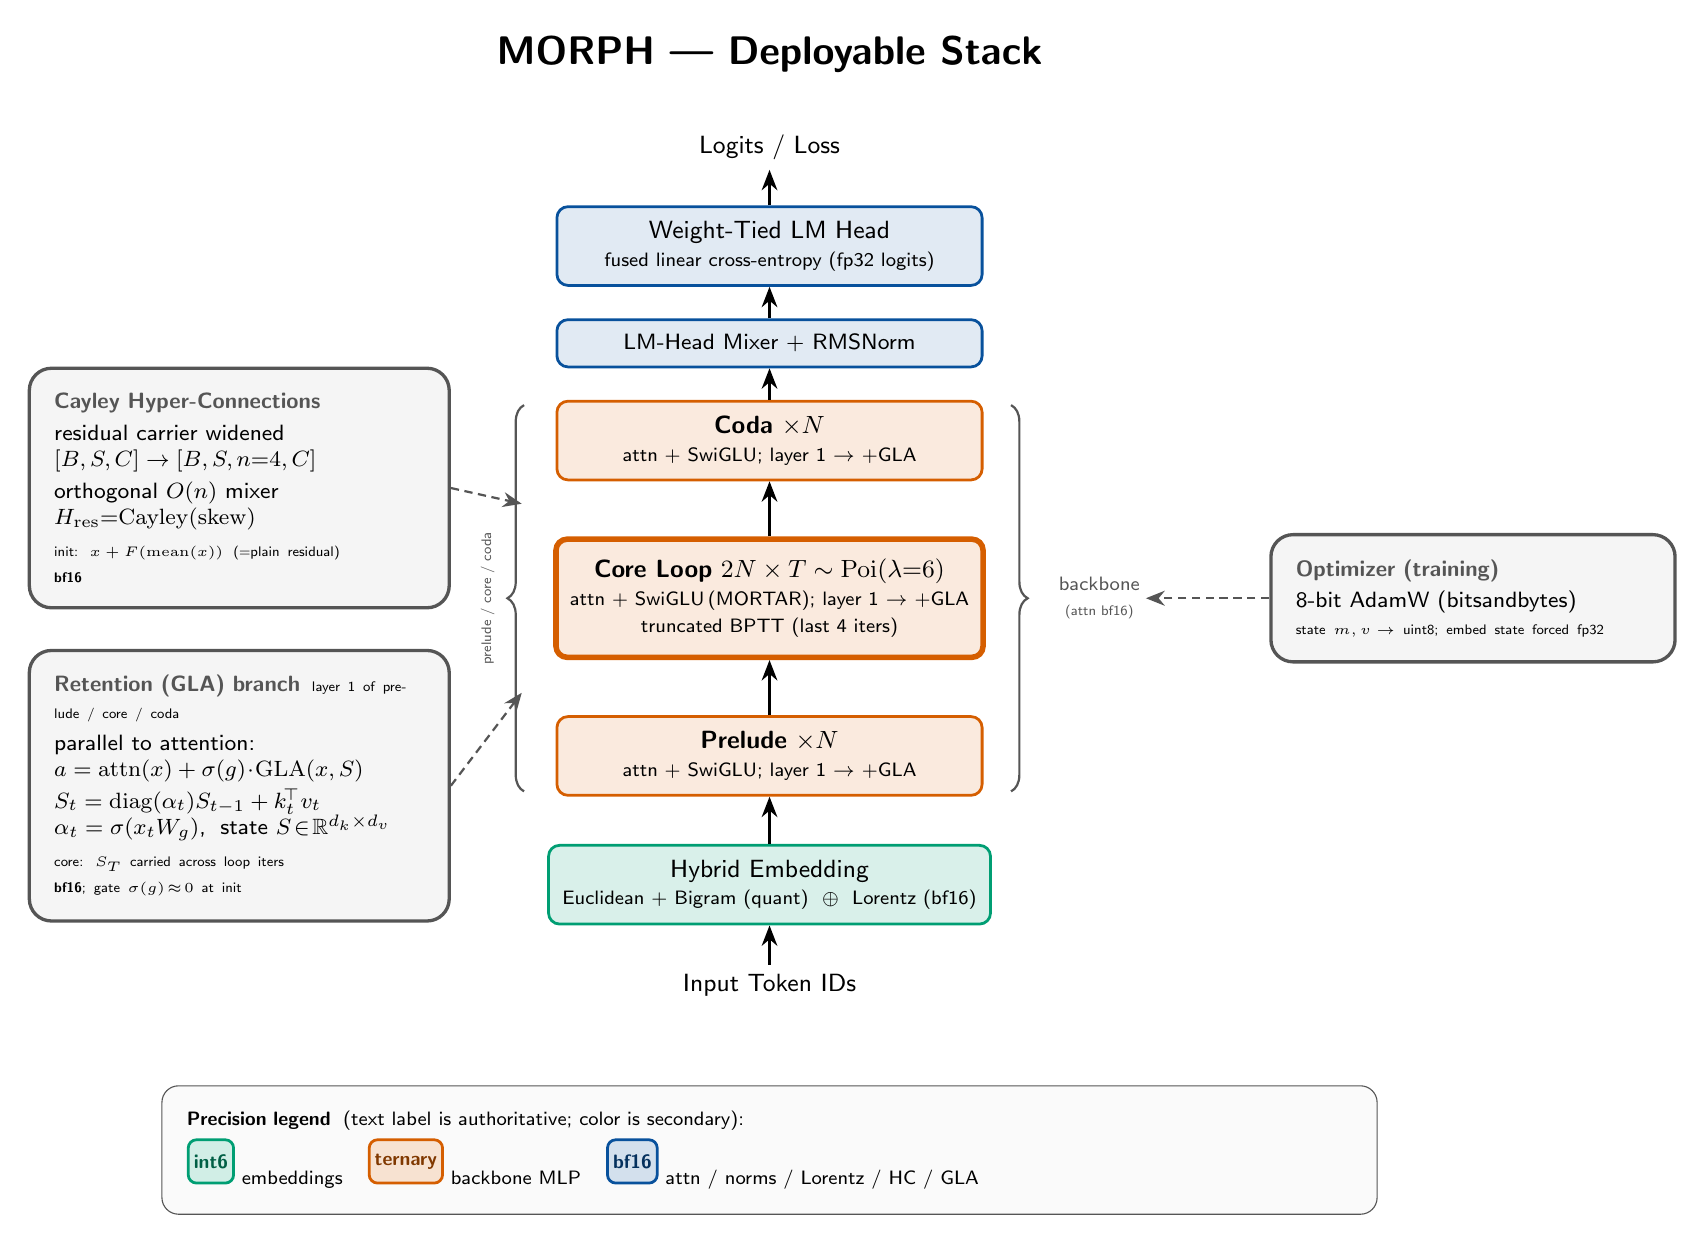
\begin{tikzpicture}[node distance=0.46cm]

% =====================================================================
% CENTRAL FORWARD-FLOW COLUMN  (input at bottom -> logits at top, matching overview)
% =====================================================================

\node[font=\small\sffamily] (inp) {Input Token IDs};

\node[PI6, above=0.5cm of inp] (emb) {
  Hybrid Embedding\\[-1pt]
  {\scriptsize Euclidean + Bigram (quant) $\;\oplus\;$ Lorentz (bf16)}};
\draw[A] (inp) -- (emb);

\node[PT, above=0.6cm of emb] (pre) {
  \textbf{Prelude} $\times N$\\[-1pt]
  {\scriptsize attn + SwiGLU; layer 1 $\to$ +GLA}};
\draw[A] (emb) -- (pre);

% ── CORE LOOP (the heart) ────────────────────────────────────────────
\node[PT, above=0.7cm of pre, minimum height=1.5cm, line width=2pt] (core) {
  \textbf{Core Loop} $2N \times T \sim \mathrm{Poi}(\lambda{=}6)$\\[-1pt]
  {\scriptsize attn + SwiGLU\,(MORTAR); layer 1 $\to$ +GLA}\\[-1pt]
  {\scriptsize truncated BPTT (last 4 iters)}};
\draw[A] (pre) -- (core);

\node[PT, above=0.7cm of core] (coda) {
  \textbf{Coda} $\times N$\\[-1pt]
  {\scriptsize attn + SwiGLU; layer 1 $\to$ +GLA}};
\draw[A] (core) -- (coda);

\node[PBs, above=0.4cm of coda] (mix) {LM-Head Mixer + RMSNorm};
\draw[A] (coda) -- (mix);

\node[PB, above=0.4cm of mix] (head) {
  Weight-Tied LM Head\\[-1pt]{\scriptsize fused linear cross-entropy (fp32 logits)}};
\draw[A] (mix) -- (head);

\node[font=\small\sffamily, above=0.45cm of head] (out) {Logits / Loss};
\draw[A] (head) -- (out);

% ── backbone precision: ONE brace spanning prelude->coda (all 3 sections identical) ──
\draw[decorate, decoration={brace, amplitude=6pt}, thick, bdr]
  ($(coda.east)+(0.35,0.45)$) -- ($(pre.east)+(0.35,-0.45)$);
\node[anchor=west, font=\scriptsize\sffamily, align=center, text=bdr,
      inner sep=2pt] (bb) at ($(core.east)+(0.85,0)$) {%
  backbone\\[1pt]{\tiny (attn bf16)}};

% =====================================================================
% LEFT PANEL — architecture carriers (cross-cutting, all bf16)
% =====================================================================

\node[panel=bdr, anchor=east, text width=4.7cm] at ($(core.west)+(-1.3,1.4)$) (hc) {
  \textbf{\textcolor{bdr}{Cayley Hyper-Connections}}\\[2pt]
  residual carrier widened\\
  $[B,S,C] \to [B,S,n{=}4,C]$\\[2pt]
  orthogonal $O(n)$ mixer\\
  $H_{\mathrm{res}}{=}\mathrm{Cayley}(\mathrm{skew})$\\[2pt]
  {\tiny init: $x + F(\mathrm{mean}(x))$ \,(=plain residual)}\\
  {\tiny \textbf{bf16}}};

\node[panel=bdr, anchor=east, text width=4.7cm, below=0.5cm of hc] (gla) {
  \textbf{\textcolor{bdr}{Retention (GLA) branch}} \,{\tiny layer 1 of prelude / core / coda}\\[2pt]
  parallel to attention:\\
  $a = \mathrm{attn}(x) + \sigma(g)\!\cdot\!\mathrm{GLA}(x,S)$\\[2pt]
  $S_t = \mathrm{diag}(\alpha_t)S_{t-1} + k_t^{\!\top} v_t$\\
  $\alpha_t = \sigma(x_t W_g)$,\; state $S\!\in\!\mathbb{R}^{d_k\times d_v}$\\[2pt]
  {\tiny core: $S_T$ carried across loop iters}\\
  {\tiny \textbf{bf16}; gate $\sigma(g)\!\approx\!0$ at init}};

% left brace spanning prelude->coda: BOTH carriers apply across the whole backbone,
% not just the core loop (HC = every layer; GLA = layer 1 of each of the 3 sections)
\draw[decorate, decoration={brace, amplitude=6pt, mirror}, thick, bdr]
  ($(coda.west)+(-0.4,0.45)$) -- ($(pre.west)+(-0.4,-0.45)$);
\node[font=\tiny\sffamily, text=bdr, rotate=90, anchor=south]
  at ($(core.west)+(-0.62,0)$) {prelude / core / coda};
\draw[Ad, bdr] (hc.east) -- ($(core.west)+(-0.4,1.2)$);
\draw[Ad, bdr] (gla.east) -- ($(core.west)+(-0.4,-1.2)$);

% =====================================================================
% RIGHT PANEL — train-time / inference-time overlays
% =====================================================================

\node[panel=bdr, anchor=west, text width=4.5cm] at ($(core.east)+(3.6,0)$) (opt) {
  \textbf{\textcolor{bdr}{Optimizer (training)}}\\[2pt]
  8-bit AdamW (bitsandbytes)\\
  {\tiny state $m,v \to$ uint8; embed state forced fp32}};

% the training-time optimizer overlay connects to the backbone brace (a real target, not empty space)
\draw[Ad, bdr] (opt.west) -- (bb.east);

% =====================================================================
% BOTTOM — precision legend + validated evidence
% =====================================================================

\node[draw=bdr, rounded corners=6pt, fill=fGray!25, inner sep=9pt,
      align=left, font=\scriptsize\sffamily, text width=14.8cm,
      below=1.0cm of inp, anchor=north] (leg) {
  \textbf{Precision legend} \;(text label is authoritative; color is secondary):\\[2pt]
  \tikz\node[badge=pInt6, inner sep=2pt]{int6};~embeddings \;\;
  \tikz\node[badge=pTern, inner sep=2pt]{ternary};~backbone MLP \;\;
  \tikz\node[badge=pBf16, inner sep=2pt]{bf16};~attn / norms / Lorentz / HC / GLA};

% ── Title ────────────────────────────────────────────────────────────
\node[above=0.55cm of out, font=\Large\sffamily\bfseries]
  {MORPH --- Deployable Stack};

\end{tikzpicture}
\end{document}
